\documentclass[main]{subfiles}

\begin{document}
    \subsection{Геодезические, их существование}
    %\begin{figure}[H]
    %    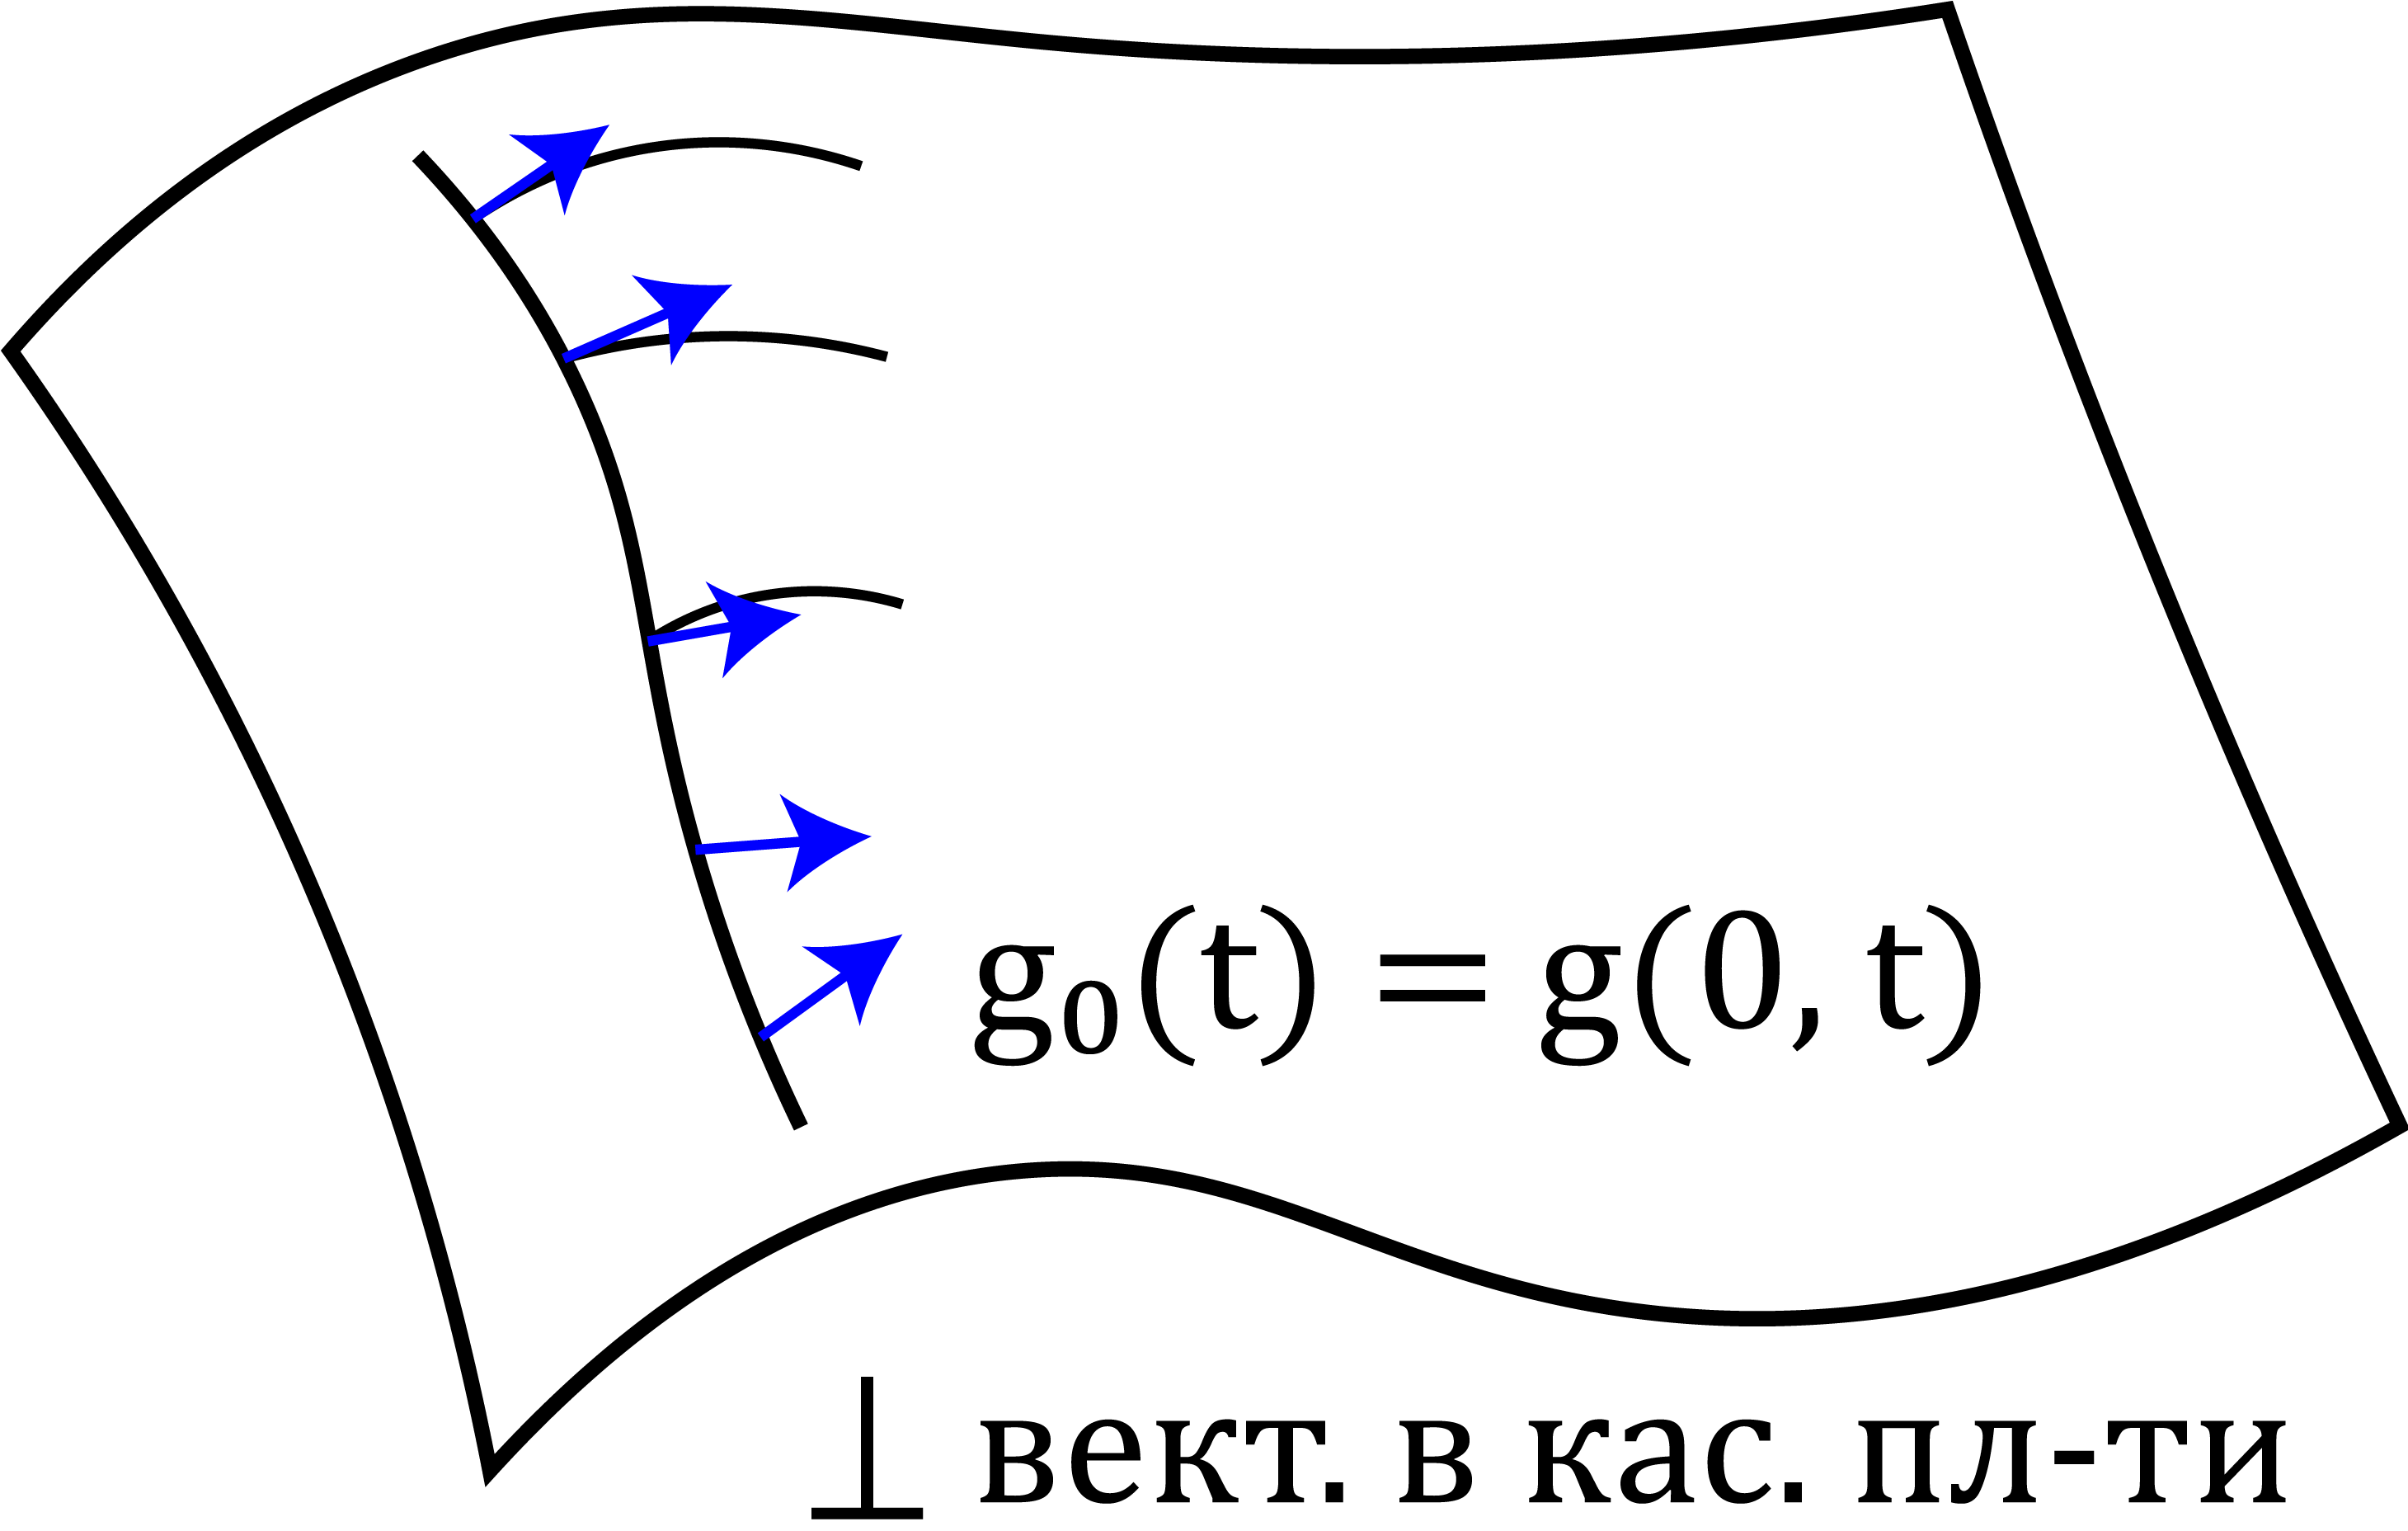
\includegraphics[width=7cm]{pics/12_1.png}
    %    \centering
    %\end{figure}
    \begin{theorem}
        Из $\forall $ точки пов-ти в $\forall $ напр можно выпустить ровно одну геодез.\\
    \end{theorem}

    \begin{advice}
        Посмотреть док-во в учебнике Александрова и Нецветаева, там подробнее
    \end{advice}

    \begin{proof}
        Из диффуров реш. $\exists $ и единств.
        \[\mathcal{E}(u, v) \q u(t) \q v(t)\]
        \[K_g = \frac{\abs{(\frac{d^2 r}{dt^2}; \frac{dr}{dt}; n)}}{\abs{\frac{dr}{dt}}^3}\]
        \[u(t) =  t\]
        \[v(t) \text{ --- функция}\]
        \[t = \varphi(u)\]
        \[v(\varphi(u))\]
        \[u' \neq 0\]
        \[\text{Хотим } (r''_{tt}; r'_{t}; n  ) = 0\]
        \[r'_t = r_u  u'_t + r_v v'_t = r_u + r_vv'\]
        \[r''_t = r_{uu}(u')^2 + 2r_{uv}u'v' + r_{vv}(v')^2 + r_u u'' + r_v v'' =\]
        \[= r_{uu} + 2r_{uv} v' + r_{vv}(v')^2 + r_v v''\]
        \[(r_{uu} + 2r_{uv}v'  + r_{vv}(v')^2 + r_v v''; r_u + r_vv'; n   ) = 0\]
        \[(r_{uu} + 2r_{uv}v' + r_{vv}v'^2; r_u + r_v v'; n) +
        (r_v v''; r_u + \us{\text{т.к 1 сомнож } \parallel r_v}{\cancel{r_v v'}}; n) = 0\]
        \[(r_v v''; r_u; n) = -v''(r_u; r_v; n)\]
        \[v'' = \frac{(r_{uu} + 2r_{uv}v' + r_{vv}v'^2; r_u + r_vv'; n   )}{(r_u; r_v; n)}\]
        \[v'' = F(v'; v; t)\]
        \[F \text{ непр}\]
        Знаменатель в ноль не обращается (существование)
        \[x' = F(x, t) \q \text{ если } F \text{ непр } \Ra \exists \text{ реш} \]
        \[\text{Если } \frac{\d F}{\d x} \neq 0  \ \Ra \  \text{единств.}\]
        \[\text{Реш } \exists  \text{ и единств.}  \]
        \[v(t_0) = v_0 \ \text{ и } \ v'(t_0) = \psi_0\]
    \end{proof}

    \subsection{Полугеодезическая параметризация}
    \begin{figure}[H]
        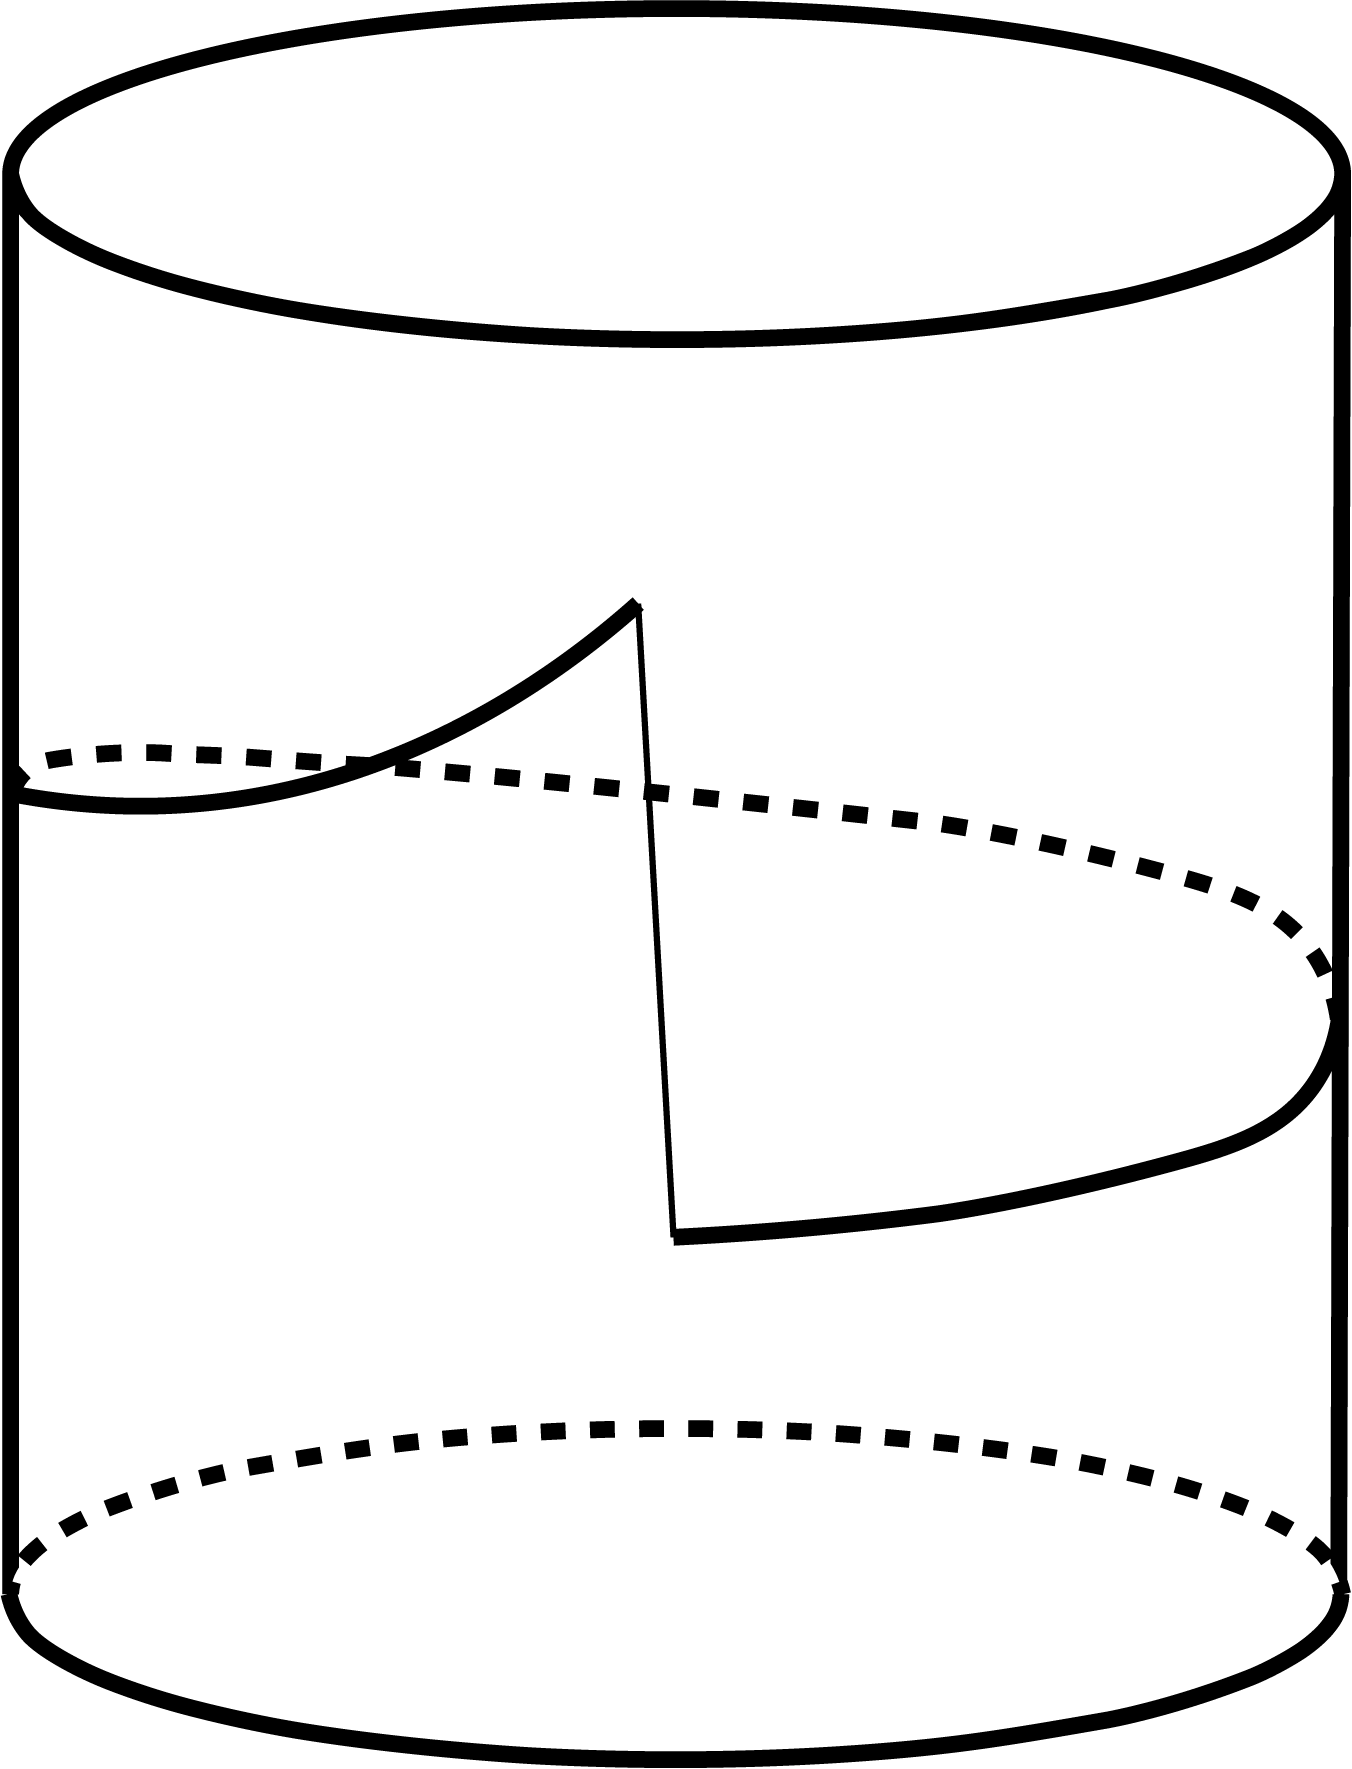
\includegraphics[width=3.5cm]{pics/12_2.png}
        \centering
    \end{figure}

    \begin{Theorem}
        \[g(s, t) \text{ --- параметр. поверхности}\]
        \[E = 1; \ F = 0\]
        \[\text{Выберем произв. кривую $g_0(t)$}\]
        \[\text{В каждой точке проведем вектор $\bot$ в касат. плоск.}\]
        \[\forall t \ \exists \text{ геодезич. в натуральной параметризации } h_{(t)} (s) \q s \in [0, \mathcal{E})\]
    \end{Theorem}

    \begin{advice}
        Посмотреть док-во в учебнике Александрова и Нецветаева, там подробнее
    \end{advice}

    \begin{Proof}
        \[g(s, t) = h_{(t)} (s)\]
        \[g(0, t) = g_0(t) = h_{(t)} (0)\]
        \[E = g_s \cdot g_s = \abs{g_s}^2 = \abs{h_{(t)s}' }^2 = 1 \text{ т.к. парам. натур.}\]
        \[F(0, t) = 0\]
        Осталось доказать, что $F_s(s, t) = 0$
        \[F_s = (g_s \cdot g_t)_s = \underbracket{g_{ss} \cdot g_t}_{=0}  + g_{st} \cdot g_s  =\]
        \[g_{ss} \text{ --- вектор кривизны } h_{(t)}(s)  \]
        \[g_t \text{ --- вектор в кас. плоск.}\]
        \[g_{ss} \perp g_t \text{ т.к. } h \text{ --- геодез.} \]
        \[= g_{st} \cdot g_s = \frac{1}{2}(g_s \cdot g_s)_t = \frac{1}{2}E_t = 0 \q \text{т.к } E = 1 \]
        Т.о в окр-ти каждой точки $\exists $ парам,
        \[\RNumb{1} \text{ форма } \q (u')^2 + G(v')^2\]
    \end{Proof}

    \subsection{Геодезические как локально кратчайшие.}
    \begin{theorem}
        Геодез. --- локально кратчайшие
    \end{theorem}

    \begin{advice}
        Посмотреть док-во в учебнике Александрова и Нецветаева
    \end{advice}

    \begin{proof}
        Введем полугеодез. коорд.
        %рисунок3
        \begin{figure}[H]
            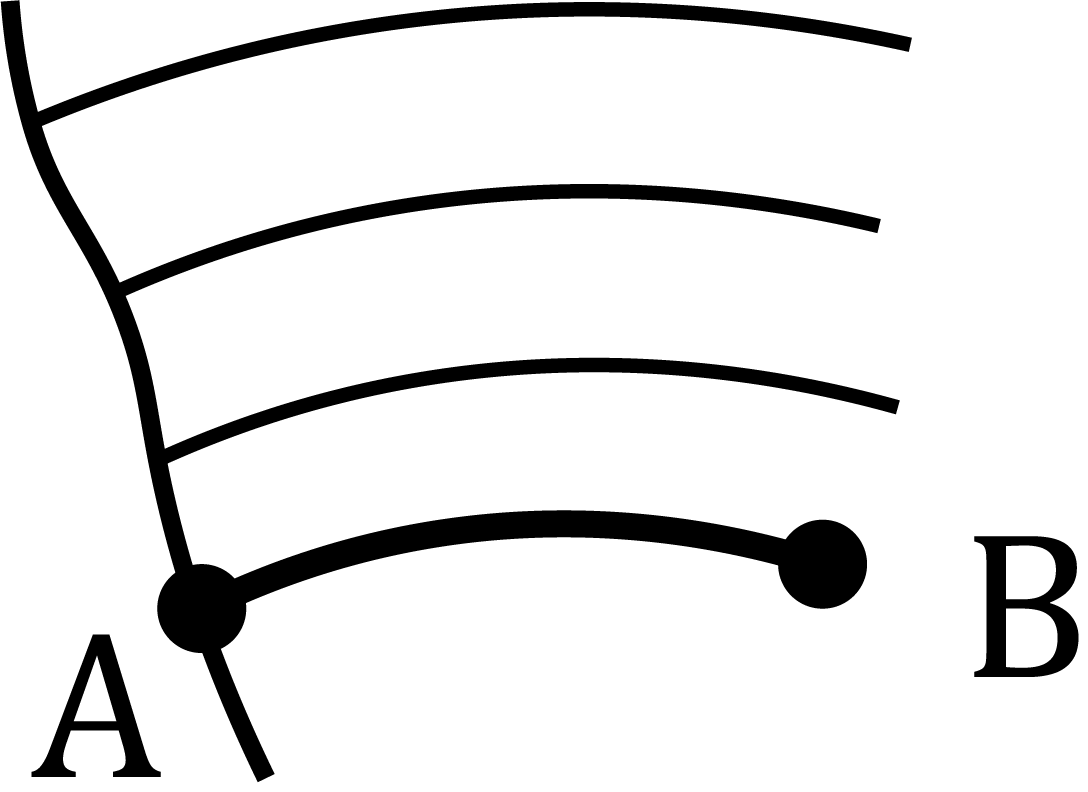
\includegraphics[width=3cm]{pics/12_3.png}
            \centering
        \end{figure}
        \[g(s, t) \q A(0, 0), \q B(s_1, 0)\]
        \[l_{\us{\forall \text{ кривая}}{AB}} = \int_{\tau_0}^{\tau_1}   \sqrt{Es'^2 + 2Fs't' + Gt'^2}d\tau =
        \int_0^{s_1} \sqrt{1 + Gt'^2}dt \geq \int_0^{s_1} \sqrt{1}d\tau = s_1 \]
        \[s_1 \text{ --- длина геодез. } AB\]
        \[s(\tau); \ t(\tau)\]
        \[s(\tau) = \tau \text{ считаем так}\]
    \end{proof}

    %\begin{Theorem}
    %    \[\iint_\Phi Kds = 2\pi \int k_g ds + \sum \varphi_i  \q ??? \]
    %   %рисунок4
    %\end{Theorem}

    %\begin{Example}
    %    %рисунок5
    %    \[K = 1\]
    %    \[\iint Kds = \int_{\triangle} = \frac{1}{2}\pi \]
    %\end{Example}

    %\begin{theorem}[Гаусса - Бонне, не нужно]
    %    Если пов-ть замкн.
    %    \[\iint K ds = 2\pi \chi_\Phi\]
    %\[\chi = \text{ кол-во вершин } - \text{ кол-во ребер} + \text{  кол-во граней}\]
    %\end{theorem}

    %\begin{Example}
        %рисунок5
    %    \[\chi = 2\]
    %    \[B = 6 \q P = 12 \q \Gamma = 8 \qq 6 + 8 - 12 = 2\]
    %\end{Example}

    \newpage
    \section{Благодарность}
    Спасибо друзьям-матобесам с за многочисленные правки
    \\ \ \\
    А именно Егору Гусеву, Ладе Егоровой, Илье Вологину, Дмитрию Вологину, Николаю Мочалыгину, Екатерине Винник, Юнии Ким, Ольге Голубевой, Олегу Щербине, Захару Захарову, Александру Семенову
\end{document}
